\section{Une étude de cas : Cholesky}\label{sec:contribs:apps:cholesky}

Afin de mettre en application nos analyses nous avons choisi comme cas d'étude une application d'algèbre linéaire très étudiée et bien connue : la factorisation de Cholesky.
Une manière standard de paralléliser les applications d'algèbre linéaire est de découper le problème en l'appliquant à différentes sous parties (ou \emph{blocs}) des matrices.

Nous allons étudier en détails l'algorithme de Cholesky par blocs tel qu'implémenté dans PLASMA~\cite{Kurzak2013}, dont nous donnons le code dans le listing~\ref{lst:contribs:apps:cholesky-block-plasma}.
Nous allons voir quelles sont ses parties critiques et leurs comportements, et nous allons également voir comment nous avons pu améliorer son exécution.

\begin{figure}[h]
\begin{lstlisting}[language=c++,caption=Algorithme de Cholesky par bloc tel qu'exprimé dans PLASMA,label=lst:contribs:apps:cholesky-block-plasma]
for (int k = 0; k < n_blocs; k++) {
  DPOTRF(A(k, k));

  for (int m = k+1; m < n_blocs; m++) {
    DTRSM(A(k, k), A(k, m));
  }

  for (int m = k+1; m < n_blocs; m++) {
    DSYRK(A(k, m), A(k, k));

    for (int n = k+1; n < m; n++) {
      DGEMM(A(k, n), A(k, m), A(n, m));
    }
  }
}
\end{lstlisting}
\end{figure}


\subsection{Description générale}

La factorisation de Cholesky a pour but de résoudre l'équation suivante :

$$ A = L*L^T$$

Où $A$ est une matrice symétrique définie positive à coefficients réels, et $L$ est l'inconnue, une matrice triangulaire inférieure.

Pour paralléliser la résolution de cette équation, nous allons découper la matrice $A$ par bloc, et appliquer un algorithme de Cholesky par bloc.
Nous pouvons donc caractériser une factorisation de Cholesky par sa taille de bloc et sa largeur en nombre de blocs.

L'algorithme de résolution par bloc repose sur quatre algorithmes basiques d'algèbre linéaire tirés des \emph{BLAS} - \emph{Basic Linear Algebra Subprograms} - décrits ci-dessous~:


\paragraph{\potrfcolor{POTRF(A)}}

Ce noyau effectue la factorisation de Cholesky de base sur une matrice symétrique définie positive $A$.

\paragraph{\trsmcolor{TRSM(A, B)}}

Ce noyau résoud l'équation suivante~: $A*X = B$, où $A$ est une matrice triangulaire, et $B$ une matrice générique. $B$ est écrasée par la matrice solution $X$.

\paragraph{\syrkcolor{SYRK(A, C)}}

Ce noyau effectue l'opération suivante~: $C := A*A^t + C$, où $A$ est une matrice générique, et $C$ est une matrice symétrique.

\paragraph{\gemmcolor{GEMM(A, B, C)}}

Ce noyau effectue une multiplication de matrices génériques, définie de la manière suivante~: $C := A*B + C$, où $A$, $B$, et $C$ sont des matrices génériques.

\begin{figure}[h]
  \centering
  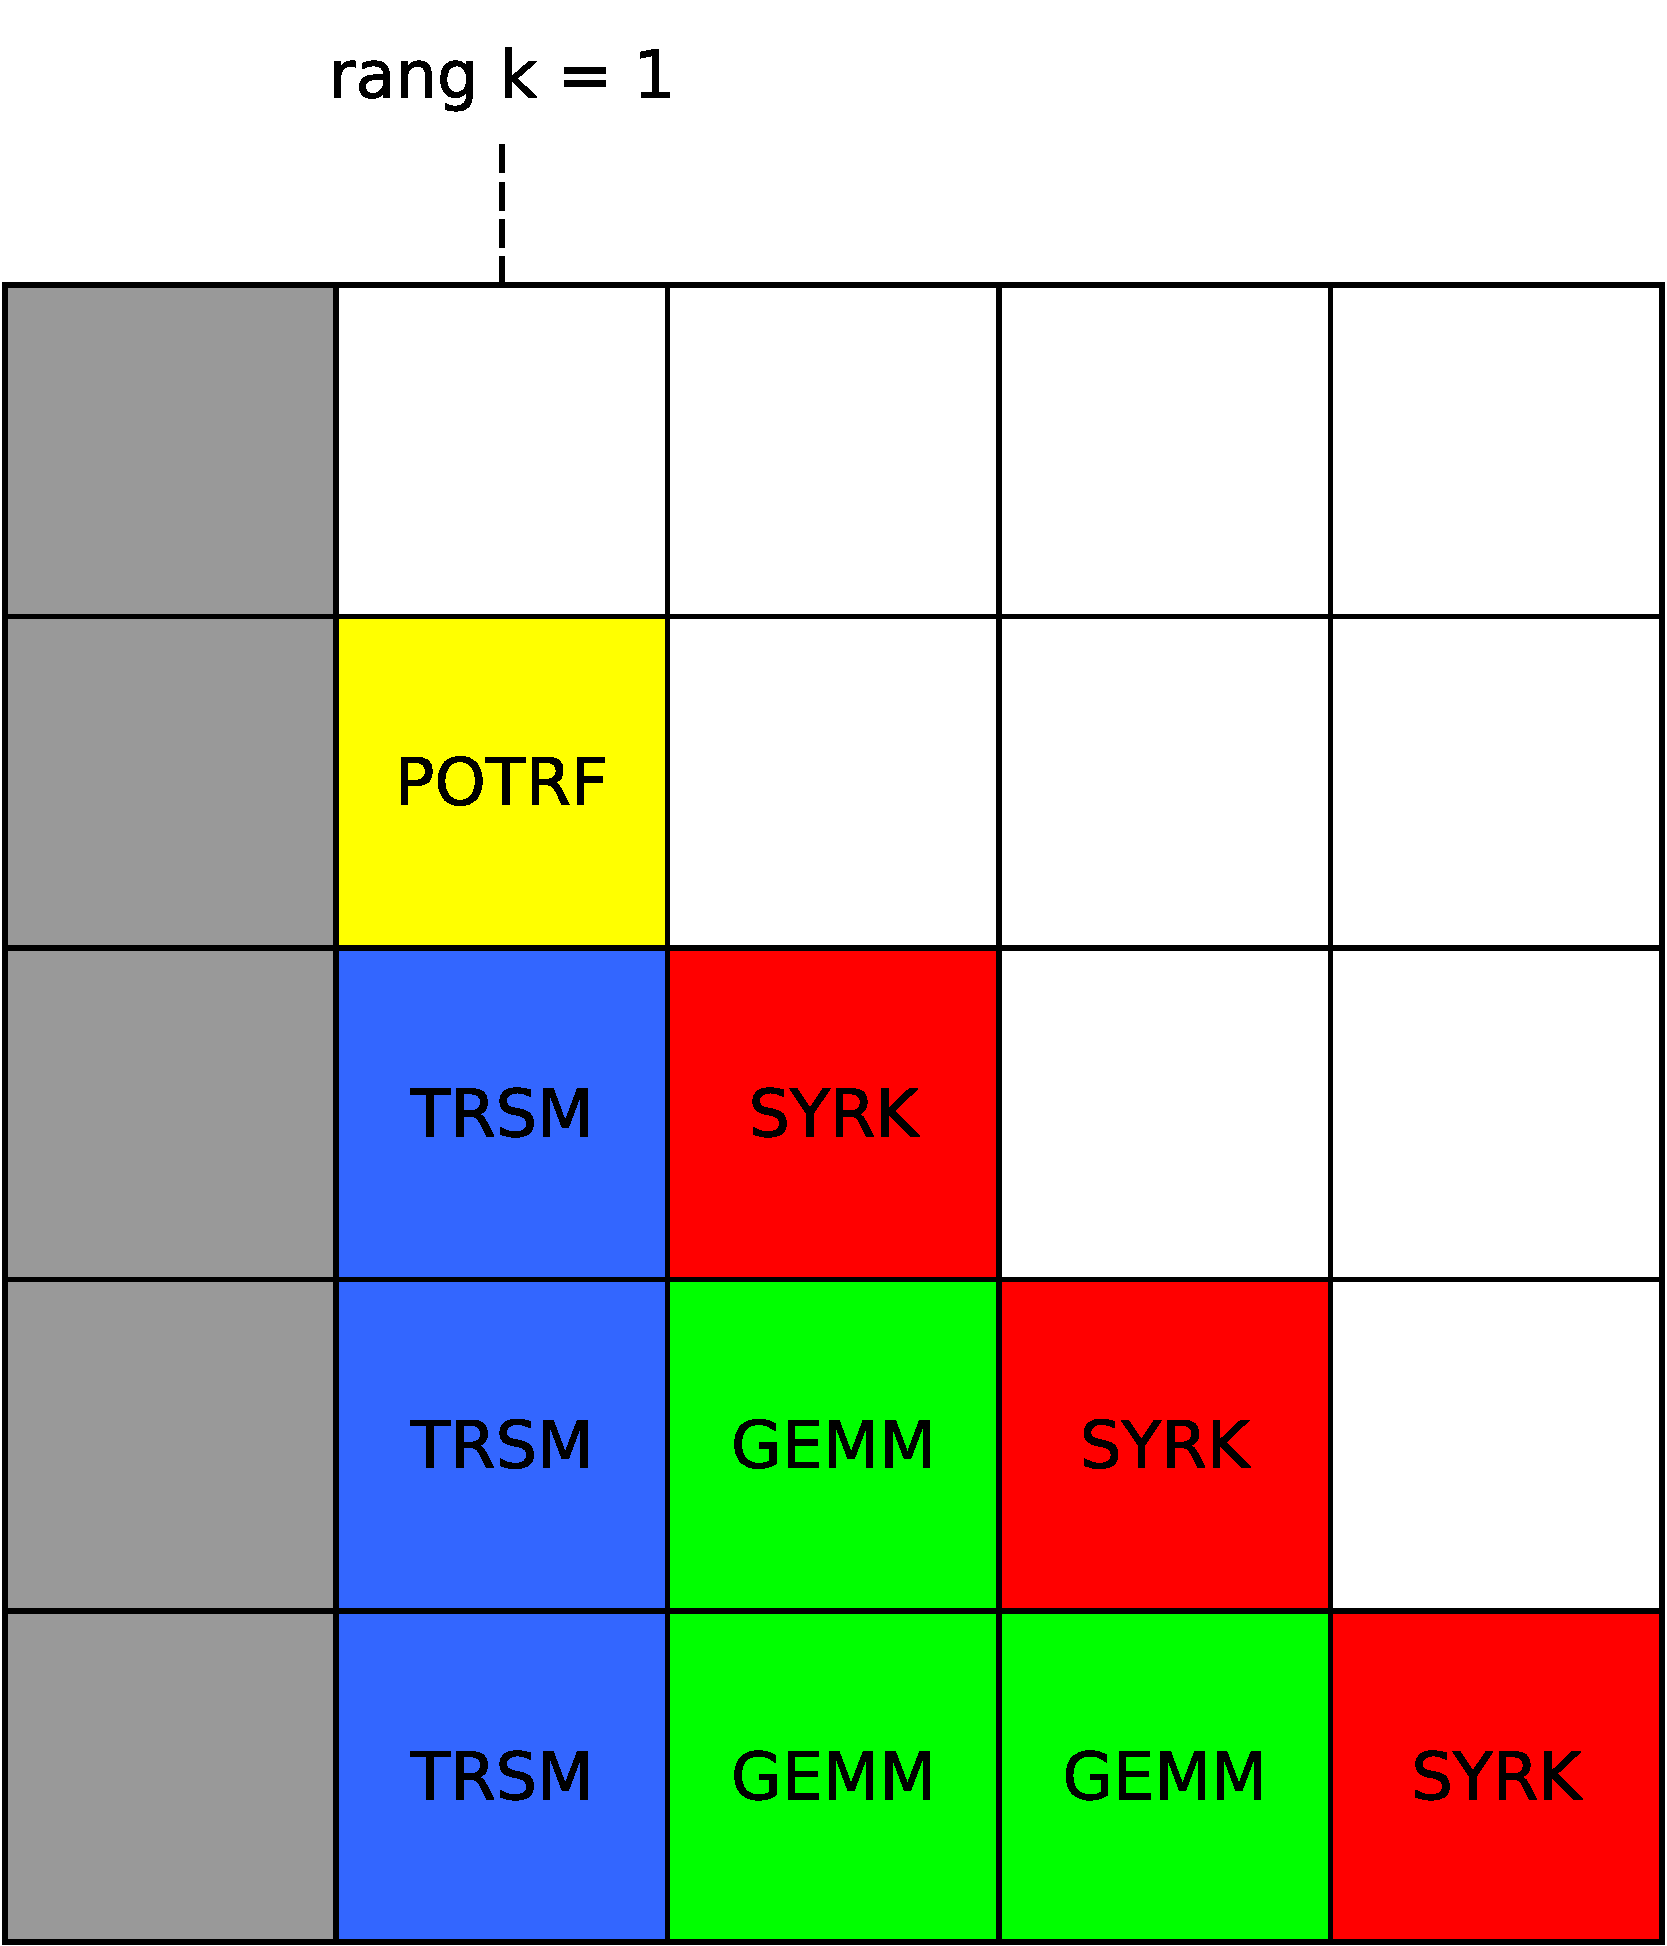
\includegraphics[width=0.6\textwidth]{cholesky-rank-update}
  \caption{Itération du rang k de la factorisation de Cholesky}\label{fig:contribs:apps:cholesky:rank-update}
\end{figure}

Pour permettre de mieux représenter l'algorithme du listing~\ref{lst:contribs:apps:cholesky-block-plasma}, les opérations se produisant sur chaque bloc de la matrice au rang |k| sont illustrées sur la figure~\ref{fig:contribs:apps:cholesky:rank-update}


À chaque itération, un \potrf est d'abord effectué sur le bloc diagonal de l'itération. Les blocs de la colonne sont ensuite mis à jour via des \trsm, à la suite desquels les autres blocs restant peuvent être mis à jour par des \gemm (ou \syrk pour les blocs diagonaux).
Le parallélisme de l'algorithme est donc principalement libéré par les \potrf ainsi que les \trsm.
Cela peut être illustré par la Figure~\ref{fig:contribs:apps:cholesky:dag-5}, qui donne le graphe de dépendances d'une factorisation de Cholesky de largeur 5.

\begin{figure}[h]
  \centering
  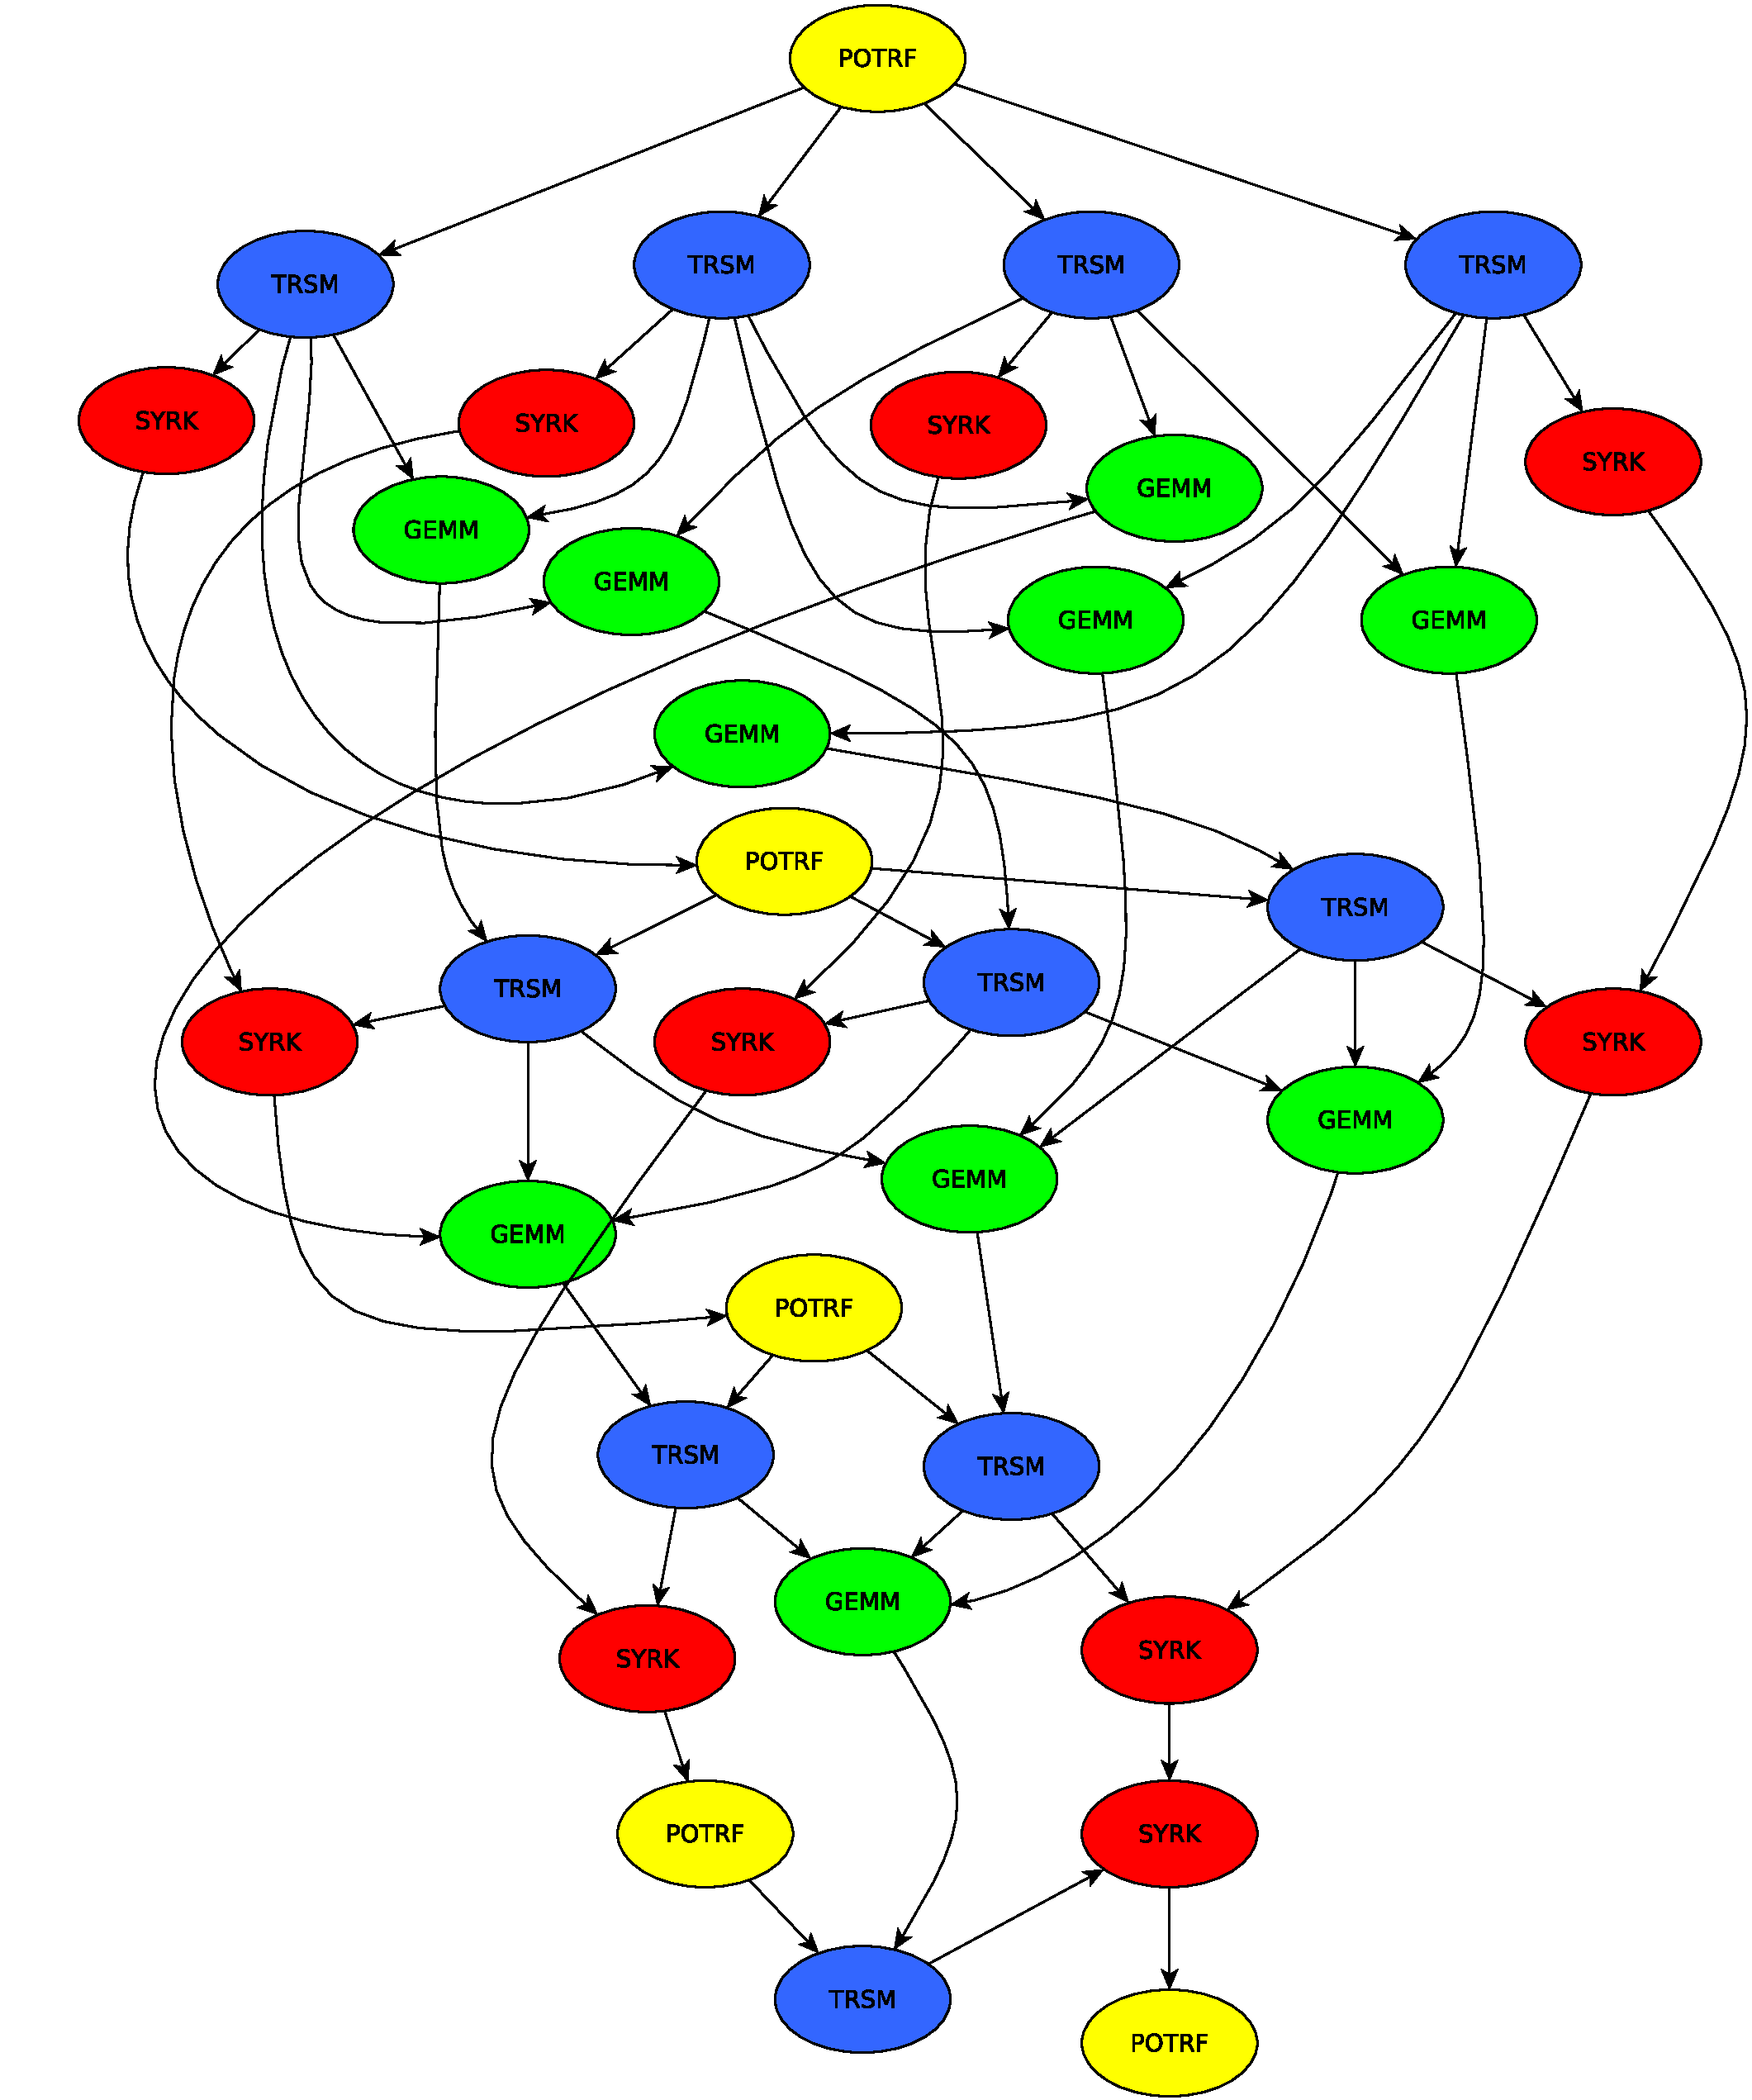
\includegraphics[width=0.7\textwidth]{cholesky-dag-5}
  \caption{DAG d'un Cholesky de largeur 5}\label{fig:contribs:apps:cholesky:dag-5}
\end{figure}

Le nombre de tâches créées pour une largeur de matrice $L$ (en nombre de blocs), le nombre d'opérations arithmétiques flottantes (ou \emph{flops}) en fonction de la taille de bloc $N$, ainsi que l'intensité opérationnelle\footnote{Définie par $\frac{Flops}{bytes}$} sont résumés dans la table~\ref{tab:contribs:apps:cholesky:kernels-info}.


\begin{table}[h!]
\def\arraystretch{1.5}
\centering
\begin{tabular}{|c||c|c|c|}\hline
  Noyau & \makecell{Nombre pour une\\largeur de matrice $L$} & \makecell{Flops pour une\\ taille de bloc $N$~\cite{LAWN41}} & \makecell{Intensité\\Opérationnelle} \\ \hline
  \potrf & $L$ & $\frac{N^3}{3} + \frac{N^2}{2} + \frac{N}{6}$ & $\frac{N}{24} + o(N)$ \\ \hline
  \trsm & $\frac{L*(L-1)}{2}$ & $N^3$ & $\frac{N}{8} + o(N)$ \\ \hline
  \syrk & $\frac{L*(L-1)}{2}$ & $N^2*(N+1)$ & $\frac{N}{8} +o(N)$ \\ \hline
  \gemm & $\frac{L^3}{6} - \frac{L^2}{2} + \frac{L}{3} + 1$ & $2*N^3$ & $\frac{N}{4} +o(N)$ \\ \hline
%$\sum_{k=1}^{n}\frac{(k-1)*(k-2)}{2}$
%simplifié via wolframalpha
\end{tabular}
\caption{Nombre et complexité des différents noyaux}\label{tab:contribs:apps:cholesky:kernels-info}
\end{table}

Les \gemm sont donc très largement majoritaires dans l'algorithme quand la largeur de la matrice augmente.
En revanche en terme de Flops et d'intensité opérationnelle, on peut constater que tous les noyaux présentent des chiffres d'un ordre de grandeur équivalent.


\subsection{Observations préliminaires et limites}\label{sec:contribs:apps:cholesky:observations}

Cette section et les suivantes montrent des évaluations reposant sur une bibliothèque BLAS, sauf indication contraire, la version utilisée est OpenBLAS 2.19.
La figure~\ref{fig:context:granularity} a montré qu'on pouvait observer l'impact de certains paramètres, tels que la taille de bloc ou le support exécutif, sur les performances globales.

Certains supports exécutifs tels que Kaapi, StarPU, OpenStream, ou encore OmpSs permettent d'aller plus loin via un système de traces, permettant d'observer certaines caractéristiques de tâches particulières.

\begin{figure}[t!]
  \centering
  \includegraphics[width=\textwidth]{graph_evolution_cholesky_8192_224}
  \caption{Évolution des performances de Cholesky avec libKOMP, pour une taille de matrice de 8192 et une taille de bloc de 224}\label{fig:contribs:apps:cholesky:overview-8192-224}
\end{figure}

Pour illustrer cela, prenons un exemple d'évolution des performances de Cholesky en fonction du nombre de cœurs utilisés, montré sur la figure~\ref{fig:contribs:apps:cholesky:overview-8192-224}. Dans cet exemple la taille de matrice est de 8192, la taille de bloc de 224, et le support exécutif utilisé est libKOMP, sans aucune extension relatives à nos travaux sur l'affinité des données, que nous présentons dans le chapitre~\ref{chap:contrib:openmp}.

En activant le support des traces, on peut avoir plus de détails sur l'exécution individuelle de chacune des tâches.

\begin{figure}[h!]
  \centering
  \includegraphics[width=\textwidth]{graph_distrib_overview_8192_224}
  \caption{Distribution des différents noyaux en fonction du nombre de cœurs}\label{fig:contribs:apps:cholesky:distrib-overview-8192-224}
\end{figure}

La figure~\ref{fig:contribs:apps:cholesky:distrib-overview-8192-224} montre, pour chaque type de tâche (ou \emph{noyau}), la répartition du temps d'exécution (en cycles) en fonction du nombre de cœurs.

On constate deux types de répartitions~:
\begin{itemize}
  \item Une distribution relativement restreinte des cycles de chaque noyau, typiquement observée pour 16 cœurs.
    La distribution peut avoir plusieurs pics~: pour \gemm sur 16 cœurs par exemple.
    Cela pourrait être expliqué par le nombre de cas possibles pour le placement des blocs de données manipulés par le noyau~: avec 16 cœurs il y a 2 nœuds impliqués, et donc 4 cas pour la position des blocs (3 locaux, 2 locaux, 1 local, 3 distants), ce qui pourrait correspondre aux 4 niveaux de performances observés.
  \item Une distribution relativement large, typiquement observée pour un grand nombre de cœur. Pour un \gemm sur 192 cœurs, le nombre de cycles nécessaires pour l'exécution peut varier du simple au double !
\end{itemize}

Nous souhaiterions identifier d'où vient cette évolution dans la distribution, afin d'éventuellement réussir à la corriger en limitant sa largeur.

Malheureusement il n'existait pas, à notre connaissance, d'outil permettant d'isoler une (ou plusieurs) tâches d'une application, et permettant de changer certains paramètres prédéfinis pouvant avoir un impact sur le temps d'exécution de la tâche.
Nous avons donc utilisé \outil dans le but de comprendre et d'analyser plus en profondeur nos observations préliminaires.

\subsection{Caractérisation détaillée des noyaux via \outil}\label{sec:contribs:apps:cholesky:carton}

L'objectif de cette section est de décrire le processus expérimental nous ayant permis d'analyser et comprendre le comportement des quatre noyaux de Cholesky~: \potrf, \trsm, \syrk, \gemm, qui a finalement abouti à des améliorations du support exécutif.
Nous allons donc aborder d'une part les types de scénarios exécutés via \outil, puis illustrer les résultats que nous avons obtenus avec des exemples significatifs.

\subsubsection{Description des scénarios}\label{sec:contribs:apps:cholesky:scenario}

Afin d'étudier le comportement de chaque noyau impliqué dans Cholesky, nous avons défini des scénarios au cours desquels les noyaux sont exécutés avec un contrôle sur les conditions d'exécution.

Pour un noyau donné (parmi \potrf, \trsm, \syrk, \gemm), le scénario de base est le suivant :
\begin{itemize}
  \item Allocation et initialisation des données sur un nœud précis pour une taille de bloc donnée.
  \item Exécution d'un certain nombre de répétitions du noyau choisi (par défaut 50) sur ces données, en plaçant le thread de calcul soit sur un cœur du même nœud que les données, soit sur un cœur distant.
  \item Observation de la performance en FLOPS.
\end{itemize}

Ce scénario de base est donné en entier dans l'annexe~\ref{chap:annexe:tool:dgemm-base}, pour l'exécution d'un \gemm local de taille 256.

Pour évaluer le comportement des noyaux en fonction de la charge de la machine, nous avons créé des scénarios exécutant simultanément plusieurs noyaux sur des données complètement indépendantes, et où le démarrage de l'exécution des noyaux est synchronisé.
L'annexe~\ref{chap:annexe:tool:dgemm} illustre l'un de ces scénarios, qui permet d'exécuter 8 \gemm en parallèle, sur des données locales complètement indépendantes, avec une taille de matrice de 256.

Il y a plusieurs paramètres que l'on peut faire varier pour changer les conditions d'exécution~:
\begin{itemize}
  \item Le nombre de noyaux s'exécutant simultanément~;
  \item L'utilisation de données distantes ou locales~;
  \item La taille du bloc sur lequel appliquer le noyau.
\end{itemize}

Les trois sections suivantes décrivent l'impact des changements de ces paramètres, et illustrent certaines caractéristiques des machines utilisées qui donnent des opportunités pour de possibles améliorations du support exécutif.

\subsubsection{Exécutions simultanées}

\begin{figure}[ht]
  \centering
  \includegraphics[width=0.95\textwidth]{kernel_256_local_idchire}
  \caption{Performances des noyaux (B=256) avec données locales sur idchire}\label{fig:contribs:apps:cholesky:perf-256-local}
\end{figure}

Afin d'évaluer l'impact de la charge de la machine, nous avons lancé des scénarios avec un nombre variable d'exécutions simultanées de chacun des noyaux.
Pour le remplissage de la machine, nous avons placé les exécutions linéairement sur la machine, remplissant progressivement un nœud après l'autre.

La figure~\ref{fig:contribs:apps:cholesky:perf-256-local} montre la performance moyenne (en GFlops) de chaque noyau, en fonction du nombre de cœurs exécutant simultanément des noyaux.
Par exemple pour déterminer le point d'abscisse 144 sur la figure pour un \gemm, nous avons exécuté 50 répétitions de \gemm sur chacun des 144 premiers cœurs de la machine idchire (remplissant donc les 18 premiers nœuds), de manière indépendante et simultanée.
La performance moyenne pour ce point est obtenue en faisant la moyenne des performances sur l'ensemble des exécutions.
Pour ce cas la taille de bloc a été fixée à 256, avec les données allouées et initialisées localement.

Pour une taille de bloc de 256, la quantité maximale de données utilisée par l'un des noyaux (\gemm) est de 256*256*8*3 = 1.5 Mo. La taille du cache L2 étant de 256 Ko, le jeu de données ne tient pas dans ce cache. Mais avec un nœud de 8 cœurs exécutant 8 exécutions concurrentes, la quantité totale de données utilisée serait au pire de 12.58 Mo, soit environ 50\% des 20Mo de cache L3 disponible.
On pourrait donc s'attendre à ce que la performance moyenne des noyaux ne soit impactée que par des effets locaux aux nœuds.

Néanmoins les courbes montrent clairement une dégradation des performances de chaque noyaux lorsque la charge de la machine augmente.
Ce comportement a également été observé pour d'autres tailles de blocs. Sur brunch le comportement a été également observé, avec néanmoins une dégradation moindre.

\begin{todo}
  faire la mesure via hubstat pour confirmer ou infirmer l'hypothèse de la cohérence.

  %https://www.researchgate.net/profile/Daniel_Molka/publication/315703632_Performance_Analysis_of_Complex_Shared_Memory_Systems/links/58dd3cf292851cd2d3d9d5d3/Performance-Analysis-of-Complex-Shared-Memory-Systems.pdf
  %https://pdfs.semanticscholar.org/67cf/1189c859d66bac309f9438df434fb651f97a.pdf
  % sandy bridge : https://tu-dresden.de/zih/forschung/ressourcen/dateien/abgeschlossene-projekte/benchit/2014_MSPC_authors_version.pdf?lang=en
  % haswell : https://pdfs.semanticscholar.org/67cf/1189c859d66bac309f9438df434fb651f97a.pdf
\end{todo}

\subsubsection{Impact de la localité des accès}\label{sec:contribs:apps:cholesky:locality}

Les expériences de bande passante dans la section précédente ont montrées des différences significatives dans les temps d'accès à la mémoire locale et distante.
Nous avons donc déroulé des scénarios avec des noyaux utilisant des données distantes ou des données locales afin de pouvoir les comparer, et éventuellement déceler des comportements typiques.
Lorsque les données sont dites <<locales>>, l'ensemble des données est allouée sur le nœud local. Lorsque les données sont dites <<distantes>>, l'ensemble des données est alloué sur le nœud suivant (numériquement) dans la hiérarchie de la machine.

\begin{figure}[t!]
  \centering
  \includegraphics[width=0.95\textwidth]{kernel_512_remote_idchire}
  \caption{Performances GEMM, POTRF (B=512) avec données distantes sur \emph{idchire}}\label{fig:contribs:apps:cholesky:perf-512-remote-idchire}
\end{figure}
\begin{figure}[h!]
  \centering
  \includegraphics[width=0.95\textwidth]{kernel_512_remote_brunch}
  \caption{Performances GEMM, POTRF (B=512) avec données distantes sur \emph{brunch}}\label{fig:contribs:apps:cholesky:perf-512-remote-brunch}
\end{figure}

Les figures~\ref{fig:contribs:apps:cholesky:perf-512-remote-idchire} et~\ref{fig:contribs:apps:cholesky:perf-512-remote-brunch} illustrent les performances de deux noyaux, \gemm et \potrf, exécutés en concurrence sur des blocs de 512, en fonction du type d'accès, sur idchire et brunch, respectivement.

Avec une telle taille de bloc, l'ensemble des données pour tous les \potrf tient dans le cache L3, mais ce n'est pas le cas pour \gemm.
Pour les \potrf la dégradation de performances est moindre : les données tiennent dans le cache L3, il y a donc un coût pour rapatrier les données, mais une fois les données dans le cache L3 il n'y a plus besoin de faire d'accès distants.

Pour les \gemm, une utilisation de seulement quelques cœurs ne montre pas une différence de performances flagrante, en revanche le lien en sortie de nœud arrive assez vite à saturation (voir section~\ref{sec:contribs:machines:idchire:liens}), ce qui entraine une dégradation massive de performances.
À la fois pour idchire et brunch, on peut observer l'impact de la bande passante sur les performances~: les exécutions sont placées de manière à remplir progressivement les différents nœuds de la machine, et on peut observer que les courbes sont en dent de scie avec une période égale à la taille des nœuds sur chaque machine (8 sur idchire, 24 sur brunch).

Cela devient évident lorsqu'on regarde plus en détail le passage d'un nœud à un autre.
Sur la figure~\ref{fig:contribs:apps:cholesky:perf-512-remote-brunch}, la courbe pour les \gemm distants remonte progressivement entre 24 et 36 cœurs utilisés~: le fait de faire la moyenne des noyaux sur l'ensemble des cœurs cache légèrement le phénomène de saturation du lien.
En revanche ce phénomène devient évident lorsque l'on affiche la moyenne du temps d'exécution par cœurs pour certains des points de la courbe, comme illustré sur la figure~\ref{fig:contribs:apps:cholesky:distrib-load-512}.

\begin{figure}[ht]
  \centering
  \includegraphics[width=0.95\textwidth]{illustration_load_avg}
  \caption{Distribution des performances de chaque noyau (Bloc = 512), en fonction du nombre total d'exécutions concurrentes, sur brunch.}\label{fig:contribs:apps:cholesky:distrib-load-512}
\end{figure}

Le premier panneau montre la distribution des \gemm et des \potrf pour une exécution sur 24 cœurs concurrents situés sur le même nœud.
Cette distribution montre un unique pic bien défini pour chaque noyau (environ 12.5 GFlops pour \potrf, et 16.5 pour \gemm).
En revanche le passage à 26 cœurs (avec donc 2 cœurs situés seuls sur un autre nœud), montre une distribution avec deux pics~: un pic important correspondant au 24 premiers cœurs, et un second pic plus petit, montrant des performances beaucoup plus grandes, pour les 2 cœurs situé sur l'autre nœud.
Les autres panneaux montrent l'évolution de ces pics pour arriver au panneau 48, où les deux nœuds sont complètement utilisés.

%Note : Ici il y a aussi deux pics sur le panneau 48. Cela doit venir de la manière dont j'ai initialisé les accès distants : le premier nœud utilise des données du deuxième nœud, qui utilise des données du troisième nœud. Donc en pratique les liens du deuxième nœuds sont plus utilisés que ceux du premier : il doit donc un peu peiner à fournir les données nécessaires au premier nœud, ce qui expliquerait pourquoi il y a deux groupes de perf.


L'impact de la localité des données est majeur dans le cas où le jeu de données manipulé par l'ensemble des cœurs ne tient pas dans les caches L3.
Étant donné que la plus grande proportion des noyaux de Cholesky manipule 2 ou 3 blocs, la dégradation de performance devrait être importante lorsque la taille de bloc dépasse environ 320.

% Note : à la fois sur brunch et idchire, chaque cœur peut utiliser environ 2.5Mo de cache L3



\subsubsection{Impact de la taille de bloc}

La figure~\ref{fig:contribs:apps:cholesky:perf-multiple-bs-idchire} montre la performance des \gemm et \potrf sur idchire en fonction de la taille de bloc et du nombre de cœurs utilisés (tous les accès sont locaux).

\begin{figure}[ht]
  \centering
  \includegraphics[width=0.95\textwidth]{kernels_multiple_bs_local_idchire}
  \caption{Performances des noyaux avec données locales sur idchire}\label{fig:contribs:apps:cholesky:perf-multiple-bs-idchire}
\end{figure}

La taille de bloc n'a pas d'impact significatif sur le phénomène observé précédemment de dégradation des performances.
Elle a bien un impact sur le niveau de performance globale de chaque noyau (qui dépend de l'implémentation des BLAS), mais le comportement général de chaque noyau reste le même.

Cette conclusion est similaire lors d'un placement distant des données.


\subsubsection{Impact de la bibliothèque BLAS}

Pour comparer l'impact potentiel de la bibliothèque implémentant les BLAS, nous avons configuré \outil pour qu'il utilise soit OpenBLAS (2.19), Intel MKL (11.3), ou ATLAS (3.10.3).
La figure~\ref{fig:contribs:apps:cholesky:perf-blas} montre la performance des \gemm et \potrf sur \emph{brunch}, pour une taille de bloc de 256 avec des données locales, en fonction de la bibliothèque BLAS utilisée.

\begin{figure}[ht]
  \centering
  \includegraphics[width=0.98\textwidth]{comparaison_atlas_openblas_mkl_256_local}
  \caption{Comparaison des bibliothèques BLAS sur \emph{brunch}, données locales, taille de bloc = 256}\label{fig:contribs:apps:cholesky:perf-blas}
\end{figure}

Bien qu'on puisse constater une différence de performance brute, il y a dans tous les cas une baisse (relativement faible) des performances avec l'augmentation du nombre d'exécution concurrentes, bien qu'elles soient toutes indépendantes.
Pour rappel sur \emph{brunch} chaque nœud dispose de 24 cœurs, et pour les \gemm on peut deviner une baisse sur ces 24 premiers cœurs, qui d'autant plus flagrante que la performance est grande.
Cela pourrait tout simplement s'expliquer par le fait qu'on atteint la limite de bande passante cumulée disponible sur le nœud local.
Pour les autres cas, l'impact de la bibliothèque semble concerner principalement le pic de performance de chaque noyau, sans différence majeure sur l'allure générale des courbes.

\subsection{Bilan et discussions}

La figure~\ref{fig:contribs:apps:cholesky:distrib-overview-8192-224} avait montrée, à l'aide des traces obtenues à partir d'une exécution, que nous pouvions observer une baisse et une dispersion des performances individuelles des noyaux de l'application Cholesky.
\outil nous a permis d'identifier principalement deux facteurs pouvant être à l'origine de ce phénomène~: tout d'abord une partie de la baisse de performance générale est due à la baisse de performance des noyaux qui accompagne l'augmentation de la charge de la machine.
\begin{todo}
  rappeler d'où ça vient quand c'est fait
\end{todo}
L'autre partie de cette baisse de performance, ainsi que la dispersion des temps d'exécution, peuvent être attribuées à une absence de contrôle de la localité des données au cours de l'application.
